\chapter{Marco te\'{o}rico}

\section{Fractales}

Diversos f\'{i}sicos que trabajan en m\'{u}ltiples campos han reconocido que muchas de las estructuras observadas en sus experimentos exhiben un tipo particular de complejidad geom\'{e}trica, cuya comprensi\'{o}n ha sido fuertemente influenciada por los trabajos de Benoit Mandelbrot quien llam\'{o} la atenci\'{o}n sobre las propiedades geom\'{e}tricas de diversos objetos \cite{Vicsek1992}.

Los fractales son objetos geom\'{e}tricos que presentan una estructura fragmentada y aparentemente irregular que se manifiestan en muchos contextos, tanto naturales como los copos de nieve, como art\'{i}sticos por ejemplo, en las obras de M. C. Escher, as\'{i} como en fen\'{o}menos f\'{i}sicos, \textit{vervi gratia} c\'{u}mulos de galaxias, entre otras \'{a}reas. El t\'{e}rmino fractal  proviene del lat\'{i}n \textit{fractus} que significa ``roto o quebrado'' y fue acuñada por el matem\'{a}tico polaco B. Mandelbrot, padre de los fractales.

La definici\'{o}n de fractal depende del \'{a}rea en la que se est\'{e} trabajando, sin embargo existen varias propiedades que tienen estos objetos y si alguna de ellas se cumple entonces se dice que es un objeto fractal:

\begin{itemize}
	\item Es autosimilar.
	\item Su dimensi\'{o}n de Hausdorff-Besicovich es mayor que su dimensi\'{o}n topol\'{o}gica.
	\item No es diferenciable en ning\'{u}n punto.
	\item Tiene una longitud o complejidad infinita.
\end{itemize}

La  propiedad mas importante en fractales es la autosimilitud. La autosimilitud implica observar como las mismas propiedades o caracter\'{i}sticas de un objeto se replican a distintas escalas. En fractales matem\'{a}ticos o puros como el conjunto de Mandelbrot, la autosimilitud es exactamente igual sin importar el n\'{u}mero de veces que se amplie, siempre se ver\'{a} lo mismo. A la autosimilitud anterior se le conoce como autosimilitud exacta. Otro tipo de autosimilitud, es la autosimilitud aproximada que normalmente aparece en objetos donde sus partes o conjuntos de esas partes son muy similares (aunque no ind\'{e}nticas) y en su mayor\'{i}a, aparecen en la naturaleza, como en las arterias o venas de la retina de un ojo. A diferencia de la autosimilitud exacta, la autosimilitud aproximada solo se puede replicar una cierta cantidad de veces y despu\'{e}s, se pierde esa autosimilitud.

Dicho todo lo anterior, podr\'{i}amos decir que un fractal es un objeto geom\'{e}trico en el que una misma estructura irregular o aparentemente fragmentada se repite a diferentes escalas y tamaños. 

\section{Ley de potencia} 

Existe una estrecha relaci\'{o}n entre la ley de potencia y el estudio de fractales. La ley de potencia es una relaci\'{o}n matem\'{a}tica de la siguiente forma:

\begin{equation}
	y(x) = cx^{a}
	\label{eq:3.1}
\end{equation}

Donde $c$ es una constante, $a$ es el exponente de la ley de potencias,$x$ y $y$ son las variables dependientes e independientes. La ecuaci\'{o}n \ref{eq:3.1} es una funci\'{o}n matem\'{a}tica que relaciona dos cantidades, donde la modificación en una cantidad da como resultado un cambio en la otra cantidad que es proporcional al cambio elevado a un exponente constante. Es decir, una cantidad var\'{i}a como potencia de otra. El cambio es independiente del tamaño inicial de dichas cantidades \cite{Meakin1998}.

\color{blue}

\section{Dimensi\'{o}n fractal}

En geometr\'{i}a fractal existe un concepto fundamental conocido como dimensi\'{o}n fractal, que es una generalizaci\'{o}n del concepto de dimensi\'{o}n en geometr\'{i}a Euclidiana. La dimensi\'{o}n fractal $(D)$ es una medida de cu\'{a}nto aparenta llenar el espacio un objeto conforme aumentamos o disminuimos la escala de an\'{a}lisis. De la  amplia variedad de dimensiones fractales que existen, la definici\'{o}n de la dimensi\'{o}n fractal de \textit{Hausdorff-Besicovich} es probablemente la m\'{a}s usada \cite{Vicsek1992, Meakin1998}. Sin embargo, es necesario medir o calcular cantidades que puedan demostrar que est\'{a}n relacionadas con la dimensi\'{o}n fractal de los objetos que se analizan. En este contexto, existen  tres tipos de enfoques principales para la determinaci\'{o}n de la dimensi\'{o}n fractal: (1) el experimental, (2) el te\'{o}rico y (3) el inform\'{a}tico \cite{Vicsek1992}.

El enfoque inform\'{a}tico se obtienen digitalizando im\'{a}genes o por procedimientos num\'{e}ricos. Respecto a este \'{u}ltimo, los datos generados num\'{e}ricamente suelen producirse mediante variaciones del m\'{e}todo Monte Carlo y haciendo uso de datos obtenidos experimentalmente \cite{Vicsek1992}. Para hacer estimaciones precisas generalmente se calcula la dimensi\'{o}n fractal para muchos grupos y se promedia sobre los resultados. A continuaci\'{o}n hablamos de un m\'{e}todo particular para calcular $D$.

\subsection{Dimensi\'{o}n fractal de masa}
\label{masa-radio}

La dimensi\'{o}n fractal de masa es \'{u}til para estimar la dimensi\'{o}n de objetos similares como redes, vasos sangu\'{i}neos o sistemas de agregaci\'{o}n. Este m\'{e}todo consiste en seleccionar un punto que pertenece al objeto de estudio (normalmente el centro de masa) y contar el n\'{u}mero de part\'{i}culas $N$ o sitios que pertenecen al objeto dentro de una secuencia de esferas de radio $R$. La dimensi\'{o}n fractal de masa $D$ esta definida por la ley de potencia:

\begin{equation}
	M \sim R^{D}
\end{equation}


La dimensi\'{o}n fractal de masa $D$ puede calcularse ajustando una l\'{i}nea recta de los datos $\ln[N(R)]$ contra $\ln R$ dando como resultado una curva cuya pendiente asint\'{o}tica es igual a $D$, ver Figura \ref{fig:D-Fractal} . Por conveniencia, en lo que sigue usaremos con frecuencia el t\'{e}rmino part\'{i}cula para referirnos a un sitio del sistema que pertenece al fractal y \textit{cl\'{u}ster} para los objetos compuestos por part\'{i}culas conectadas \cite{Vicsek1992}.


\begin{figure}[H]
	\begin{center}
		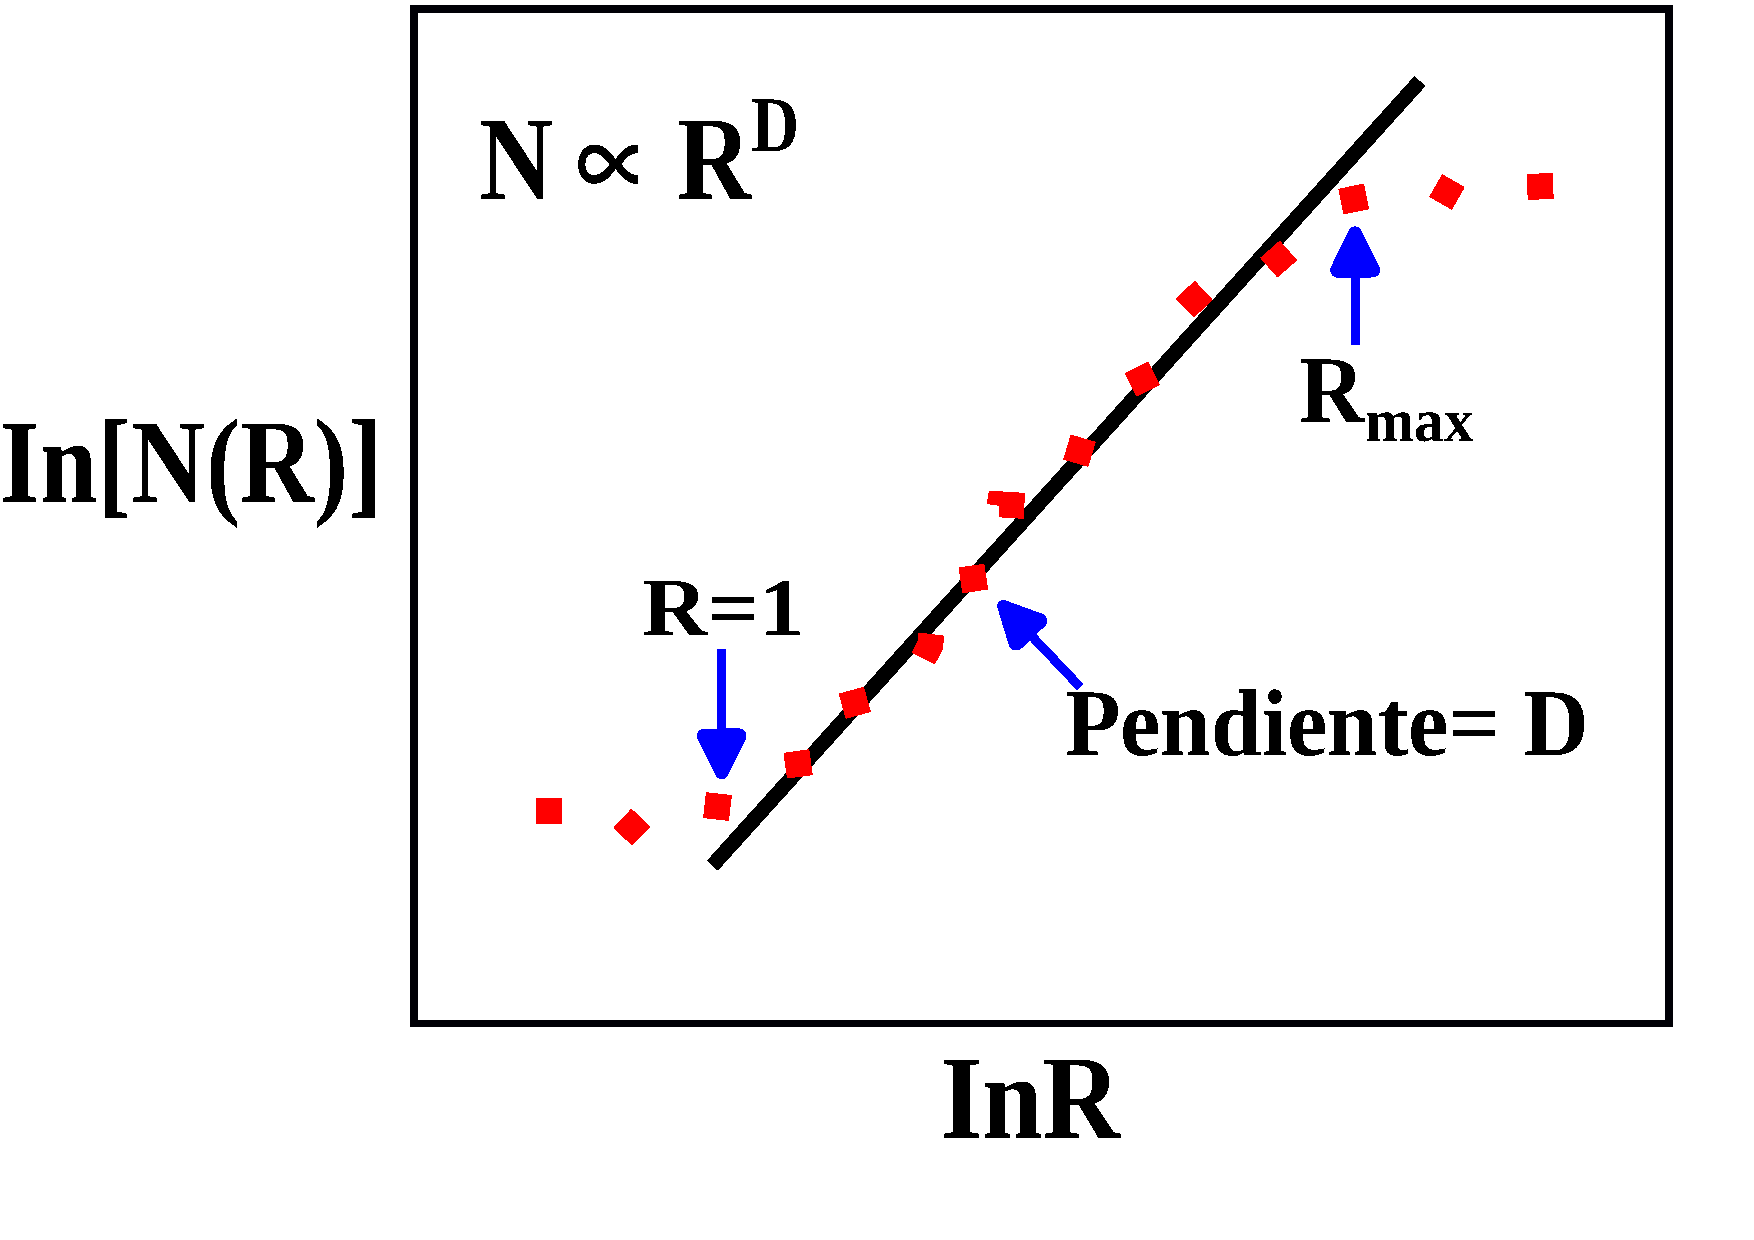
\includegraphics[width=0.5\linewidth]{graphs/dimension-fractal}
		\caption{Gr\'{a}fico de $\ln[N(R)]$ vs $\ln(R)$ del n\'{u}mero de part\'{i}culas $N(R)$ que pertenecen a un fractal que se encuentran dentro de una esfera de radio $R$. La dimensi\'{o}n fractal se obtiene ajustando una l\'{i}nea recta a los datos en la regi\'{o}n de escala.}
		\label{fig:D-Fractal}
	\end{center}
\end{figure}


\subsection*{¿Qu\'{e} es un objeto monofractal?}

Un objeto monofractal es un estructura fractal que puede describirse mediante una \'{u}nica dimensi\'{o}n fractal. Esto implica que su complejidad o irregularidad es \textbf{uniforme} en todas las escalas y regiones del objeto. Por lo tanto, su pendiente es constante y el mismo valor de dimensi\'{o}n fractal describe la estructura en todas las partes del objeto. Un caso concreto de monofractalidad es el estudio presentado por Enright \textit{et al.}\cite{Enright2005}, donde no se observa un cambio de pendiente (ve\'{a}se la Figura \ref{fig:Enright-Fractal}), probablemente por la pequeña cantidad de puntos que se presentan en su an\'{a}lisis y la distancia que hay entre los puntos. Adem\'{a}s, Enright \textit{et al.} calcul\'{o} la dimensi\'{o}n fractal de masa como un promedio espacial (usando esferas conc\'{e}ntricas y $R_g$), lo que posiblemente captura esta monofractalidad.

\begin{figure}[H]
	\begin{center}
		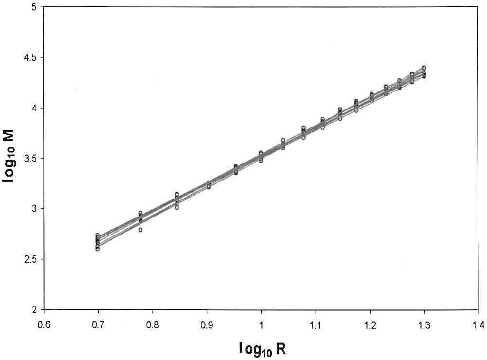
\includegraphics[width=0.6\linewidth]{graphs/Enright2005}
		\caption{Gr\'{a}fico de $\log_{10}M$ vs $\log_{10}R$ para la prote\'{i}na Sialidase, donde los valores de $M$ son las masas encerradas por esferas conc\'{e}ntricas de radio $R$ centradas en un \'{a}tomo. Imagen tomada de Enright \textit{et al} \cite{Enright2005}.}
		\label{fig:Enright-Fractal}
	\end{center}
\end{figure}

\section{Multifractalidad}

Otro concepto desarrollado por B. Mandelbrot en su libro \textit{Fractal Geometry of Nature} fue la multifractalidad. La multifractalidad es una propiedad de ciertos sistemas o estructuras complejas que presentan un crecimiento fractal pero de manera heterog\'{e}nea en distintas regiones o escalas. A diferencia de los fractales, que son descritos con una \'{u}nica dimensi\'{o}n fractal (un valor constante que representa la relaci\'{o}n entre el detalle del patr\'{o}n y la escala), en un sistema multifractalidad existen multiples dimensiones fractales que reflejan la variablidad de la distribuci\'{o}n y concentraci\'{o}n de sus elementos. 

En t\'{e}rminos simples, un sistema multifractal est\'{a} compuesto de distintas subestructuras que tienen diferentes grados de ``irregularidad'', lo que significa que cada regi\'{o}n del sistema podr\'{i}a necesitar una dimensi\'{o}n fractal espec\'{i}fica para describir su complejidad.

\section{Objetos multifractales y sistemas magnetoreol\'{o}gicos}
\label{sistemasmagneto}

Un objeto multifractal es una estructura fractal que requiere un conjunto de dimensiones fractales para ser descrita completamente. La complejidad del objeto var\'{i}a localmente y est\'{a} distribuida de manera heterog\'{e}nea, es decir, existen m\'{u}ltiples pendientes que dependen de la regi\'{o}n del objeto o de la medida que se est\'{e} analizando y es com\'{u}n en fen\'{o}menos naturales o en sistemas ca\'{o}ticos. Un ejemplo claro es el trabajo realizado por Carillo \textit{et al.} \cite{Carrillo2003}, donde los sistemas 
magnetorreol\'{o}gicos y otros conglomerados formados por procesos de agregaci\'{o}n, mostraron multifractalidad, que se manifiesta en la variaci\'{o}n de la dimensi\'{o}n fractal a lo largo de diferentes etapas del proceso de formaci\'{o}n 
de estructuras (v\'{e}ase la Figura \ref{fig:Carrillo-Fractal}). En t\'{e}rminos simples, en la Figura \ref{fig:Carrillo-Fractal}, se observa que en los puntos de $\log_{10}N(r)$ vs $\log_{10}r$ se pueden clasificar en tres conjuntos, cada conjunto sigue una relaci\'{o}n lineal con una pendiente definida, esto es, hay tres dimensiones fractales.


\begin{figure}[H]
	\begin{center}
		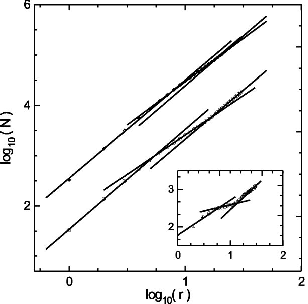
\includegraphics[width=0.5\linewidth]{graphs/Carrillo2003}
		\caption{Gr\'{a}fico de $\log_{10}N$ vs $\log_{10}r$ para estructuras formadas en un sistema magnetorreol\'{o}gico de tres etapas. La multifractalidad es una propiedad de ciertos sistemas complejos donde la estructura exhibe autosimilitud a m\'{u}ltiples  escalas. Modificado de Carrillo \textit{et al} \cite{Carrillo2003}.}
		\label{fig:Carrillo-Fractal}
	\end{center}
\end{figure}

Respecto a los sistemas magnetoreol\'{o}gicos, son fluidos complejos que contienen part\'{i}culas magn\'{e}ticas (\'{o}xidos de metales) suspendidos en un l\'{i}quido (como aceite de silicona). La caracter\'{i}stica principal de estos sistemas es que sus propiedades mec\'{a}nicas cambian dr\'{a}sticamente cuando se aplica un campo magn\'{e}tico externo. En ausencia de este campo, el fluido se comporta como un l\'{i}quido ordinario, pero al aplicar un campo magn\'{e}tico, las part\'{i}culas magn\'{e}ticas se alinean y forman estructuras organizadas (como cadenas o fibras) que transforman el fluido en una especie de gel envegecido o s\'{o}lido semirr\'{i}gido en cuesti\'{o}n de milisegundos. 


\begin{comment}
	\section{Multifractalidad en sistemas magnetoreol\'{o}gicos}
	
	Para observar los diferentes patrones de agregaci\'{o}n en presencia del campo magn\'{e}tico, Carrillo \textit{et al.} \cite{Carrillo2003} utilizaron bajas concentraciones de part\'{i}culas, de menos de 0.1 en fracci\'{o}n de volumen. Observando diferentes etapas del proceso de agregaci\'{o}n. Y por lo tanto, al determinar la dimensi\'{o}n fractal de masa observaron una variaci\'{o}n de la dimensi\'{o}n fractal que son precisamente las 3 porciones en la gr\'{a}fica que est\'{a}n asociadas a 3 etapas de agregaci\'{o}n.
\end{comment}
 
 
 
\section{Niveles de organizaci\'{o}n en la estructura de las prote\'{i}nas}


Las prote\'{i}nas est\'{a}n presentes en todos los sistemas vivos, desde estructuras como la hemoglobina o el tejido cerebral y una cantidad considerable de esas prote\'{i}nas se han cristalizado para
posteriormente, caracterizarse por m\'{e}todos como RMN, R-X, ME. Una vez hecho lo anterior, los datos son enviados y son revisados por expertos biocuradores, despu\'{e}s de
ser aprobados se ponen a disposici\'{o}n de forma gratuita bajo alg\'{u}n dominio como el \textit{Protein Data Bank} \cite{bib:Pdb-bank}.

Como es bien sabido, las prote\'{i}nas son pol\'{i}meros lineales formados por amino\'{a}cidos y aunque en la c\'{e}lula se han identificado m\'{a}s de 60 amino\'{a}cidos diferentes, solo 20 de ellos son incorporados de manera habitual en la s\'{i}ntesis de proteica.

Cada amino\'{a}cido presente en las proteínas tiene una estructura b\'{a}sica compuesta por un grupo amino (\ch{-NH2}), un grupo carboxilo (\ch{-COOH}), un \'{a}tomo de hidr\'{o}geno (\ch{-H}) y una cadena lateral o grupo R, todos ellos unidos a un \'{a}tomo de carbono central quiral (conocido como carbono $\alpha$). La uni\'{o}n covalente entre el grupo carboxilo de un amino\'{a}cido y el grupo amino de otro, con la liberaci\'{o}n de una mol\'{e}cula de agua (\ch{H2O}), da lugar al denominado enlace pept\'{i}dico, el cual constituye la base estructural de las cadenas polipept\'{i}dicas. Podemos describir a las prote\'{i}nas en cuatro niveles jer\'{a}rquicos (v\'{e}ase la Figura \ref{fig:nivelesP}):

\begin{itemize}


	\item \textbf{Estructura primaria:} Corresponde a la secuencia lineal de amino\'{a}cidos que constituyen la cadena polipept\'{i}dica. Su descripci\'{o}n especifica el orden de los amino\'{a}cidos desde el extremo amino-terminal (N-terminal) hasta el extremo carboxilo-terminal (C-terminal) de la mol\'{e}cula.
	
	\item \textbf{Estructura secundaria:} Consiste en patrones regulares y repetitivos en la disposici\'{o}n espacial local de la cadena, estabilizados principalmente por puentes de hidr\'{o}geno. Estas interacciones dan lugar a dos conformaciones secundarias principales: las $\alpha$-h\'{e}lices y l\'{a}minas $\beta$ plegadas.
	
	\item \textbf{Estructura terciaria:} Resulta de interacciones entre los grupos laterales (radicales) de los amino\'{a}cidos, los cuales presentan diversas propiedades qu\'{i}micas  (hidrofobicidad, polaridad, carga el\'{e}ctrica). Estos enlaces provocan el plegamiento, enrollamiento y torsi\'{o}n de la cadena en una conformaci\'{o}n tridimensional espec\'{i}fica, conocida como estructura nativa, que generalmente representa la configuraci\'{o}n m\'{a}s estable para una secuencia dada.
	
	\item \textbf{Estructura cuaternaria:} Es el nivel de organizaci\'{o}n que implica la asociaci\'{o}n y ensamblaje de m\'{u}ltiples cadenas polipept\'{i}dicas (subunidades) para formar una prote\'{i}na funcional. Esta estructura es caracter\'{i}stica de prote\'{i}nas oligom\'{e}ricas, com\'{u}nmente aquellas con un peso molecular superior a 50,000 uma.
\end{itemize}

\begin{figure}[H]
	\centering
	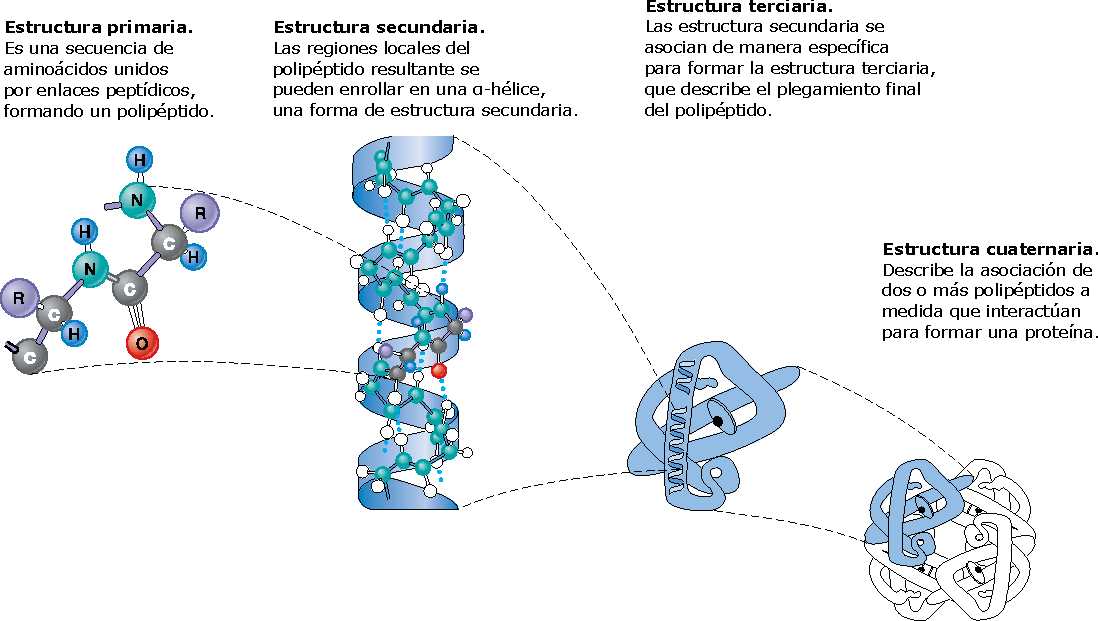
\includegraphics[width=0.7\textwidth]{graphs/niveles.pdf}
	\caption{Niveles de organizaci\'{o}n en la estructura de las prote\'{i}nas. Imagen extraida de Hardin \textit{et al.} \cite{Hardin2022}.}
	\label{fig:nivelesP}
\end{figure}

\section{Medidas para comparar estructuras proteicas}

Para evaluar y comparar estructuras proteicas a los niveles de organización proteica antes mencionados, se utilizan diferentes medidas y aunque el problema parece sencillo su cuantificaci\'{o}n es compleja y sigue evolucionando \cite{Kufareva2012}. Una de esas medidas es la desviaci\'{o}n cuadr\'{a}tica media (por su acrónimo en inglés \textit{root mean square deviation, rmsd}) es un par\'{a}metro fundamental para caracterizar transformaciones conformacionales en sistemas moleculares \cite{Santamaria2023}. Esta medida cuantifica la discrepancia estad\'{i}stica promedio entre una configuraci\'{o}n molecular en un tiempo $t$ y una estructura de referencia definida en el tiempo inicial $t_0$.

\begin{equation}
	\text{rmsd}(t) = \sqrt{ \frac{1}{N} \sum_{i=1}^{N} \left\| \mathbf{r}_i(t) - \mathbf{r}_i(t_0) \right\|^2 }
	\label{rmsd}
\end{equation}

En la ecuaci\'{o}n \ref{rmsd}, el vector \(\mathbf{r}_i(t)\) representa las coordenadas espaciales del i-\'{e}simo \'{a}tomo en el instante $t$, mientras que \(\mathbf{r}_i(t_0)\) corresponde a su posici\'{o}n de referencia. La suma se realiza sobre el conjunto de $N$ part\'{i}culas seleccionadas para el an\'{a}lisis. El uso del la \textit{rmsd} se extiende a diversas propiedades din\'{a}micas como velocidades at\'{o}micas y fuerzas interat\'{o}micas. Para comparaciones estructurales entre distintas moleculas, es necesario realizar operaciones de superposici\'{o}n geom\'{e}trica (traslaci\'{o}n y rotaci\'{o}n) que optimicen el alineamiento conformacional. En estudios proteicos, es com\'{u}n restringir el c\'{a}lculo a los carbonos $\alpha$, ya que estos forman parte de la estructura polipept\'{i}dica y proporcionan una representaci\'{o}n robusta del esqueleto proteico. Además, la evoluci\'{o}n temporal del \textit{rmsd} exhibe comportamientos diferenciados seg\'{u}n el estado de agregaci\'{o}n: en sistemas s\'{o}lidos mantiene valores reducidos pero en fase l\'{i}quida presenta un crecimiento lineal inicial que eventualmente se estabiliza tras periodos prolongados. La gr\'{a}fica que se observa en la Figura \ref{rmsd-graf} es producida mediante din\'{a}mica molecular y en ella, se estudia c\'{o}mo evolucionan las posiciones de los \'{a}tomos de una prote\'{i}na. Es importante señalar que la \textit{rmsd} es una medida  global. En la Figura \ref{rmsd-graf} no analiza si la estructura proteica se est\'{a} deshaciendo, se est\'{a} expandiendo o se est\'{a} torciendo. Solo es, cu\'{a}nto en promedio se desv\'{i}an los \'{a}tomos de su posici\'{o}n original.

	\begin{figure}[h!]
		\centering
		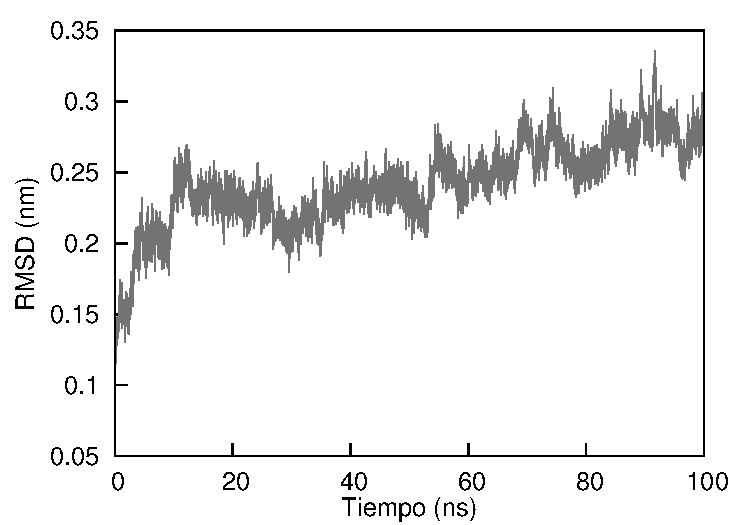
\includegraphics[width=0.8\textwidth]{graphs/rmsd.pdf}
	\caption{Gr\'{a}fica de \textit{rmsd} a 90 ns de la prote\'{i}na X.}
	\label{rmsd-graf}
	\end{figure}


Otra medida altamente utilizada es el radio de giro ($R_g$). Esta métrica describe el equilibrio conformacional (estabilidad y flexibilidad estructural) de una proteína en un entorno biológico, también evalúa la compactación de la estructura durante una simulación de dinámica molecular \cite{Saudagar2023}. Un valor pequeño de $R_g$ indica una estructura rígida, mientras que un valor alto de $R_g$, implica un incremento en la flexibilidad de la estructura. Matemáticamente, el $R_g$ se representa como:

%\begin{equation}
%	R_g = \sqrt{\frac{1}{N} \sum_{i} \left( r_i - r_{cm} \right)^2 }
%\end{equation}

\begin{equation}
	R_g = \sqrt{\frac{1}{M} \sum_{i=1}^{n} m_i \left( r_i - R \right)^2 }
	\label{rg}
\end{equation}

Donde $M$ es la masa total de la proteína, $m_i$ es la masa de cada átomo, $r_i$ es la posición de cada átomo, $R$ es el centro de masa de la proteína.

En este contexto, encontrar m\'{e}todos alternativos al \textit{rmsd} y al $R_g$ o hallar enfoques complementarios para comparar estructuras proteicas sigue siendo un reto para la comunidad cient\'{i}fica.

\subsection{Geometr\'{i}a fractal en prote\'{i}nas}
\label{Gfp}

Tras establecer la definición de dimensión fractal, multifractalidad (ver sección \ref*{sistemasmagneto}), y presentar varios métodos para su determinación. Surge la siguiente pregunta, ¿La dimensi\'{o}n fractal tiene alguna utilidad en sistemas proteicos?, la respuesta recae en varios experimentos que se ha empleado la dimensión fractal para cuantificar algunos aspectos de la morfolog\'{i}a proteica. Dado que la estructura de las prote\'{i}nas tiene una forma tan compleja, solo se puede analizar adecuadamente mediante el enfoque de la geometr\'{i}a fractal, por ejemplo se puede utilizar para caracterizar la estructura terciaria de las prote\'{i}nas y las enzimas \cite{Mustafa1996}. Aunque se pueden construir fractales iterados que son perfectamente autosimilares, la autosimilitud de una cadena de prote\'{i}nas, es similar solo en un sentido estad\'{i}stico, es decir, no siempre se ver\'{a} exactamente como el todo. Otra diferencia entre las macromol\'{e}culas biol\'{o}gicas y los objetos ideales es que una macromol\'{e}cula no es autosimilar desde culquier escala. Hay l\'{i}mites de tamaño superior e inferior m\'{a}s all\'{a} de los cuales una macromol\'{e}cula ya no es un fractal. Por lo que la investigaci\'{o}n fractal en prote\'{i}nas es un campo activo \cite{Mustafa1996}. 

\section{Metodolog\'{i}as para la determinaci\'{o}n de la dimensi\'{o}n fractal en prote\'{i}nas}

El estudio de la dimensi\'{o}n fractal en prote\'{i}nas ha evolucionado a trav\'{e}s de una combinaci\'{o}n de diferentes enfoques geom\'{e}tricos, estad\'{i}sticos y din\'{a}micos con diferentes objetivos. La diversidad de la metodolog\'{i}a en la literatura responde tanto a la disponibilidad de datos estructurales tridimensionales como a la interpretaci\'{o}n f\'{i}sica de la geometr\'{i}a fractal en sistemas moleculares complejos. A continuaci\'{o}n se muestra una breve revisi\'{o}n al estado del arte de la dimensi\'{o}n fractal en sistemas proteicos.

\subsection{Primeras aproximaciones y enfoques pioneros (1980--1990)}

Las primeras tentativas de cuantificar la naturaleza fractal de las prote\'{i}nas se remontan a los trabajos de Stapleton \textit{et al.}\cite{Stapleton1980} en 1980, quienes investigaron la estructura fractal de las prote\'{i}nas mediante estudios de relajaci\'{o}n de esp\'{i}n electr\'{o}nico con hierro (Fe$^{3+}$). Los autores midieron la dependencia t\'{e}rmica de la tasa de relajaci\'{o}n Raman y encontraron que la densidad de estados vibracionales sigue una ley de potencia. La dimensi\'{o}n fractal encontrada fue $d \approx 1.65$ que posteriormente, fue confirmada con datos de rayos X de la mioglobina. Este trabajo fue pionero en demostrar experimentalmente que las prote\'{i}nas tienen una estructura fractal. Aunque este estudio establece una base sólida para la determinación de la dimensión fractal en proteínas, no explora la multifractalidad ni variaciones locales en esas estructuras.

Cuatro años m\'{a}s tarde, Helman \textit{et al.}\cite{Helman1984} en 1984, propusieron una metodolog\'{i}a basado en la dimensi\'{o}n fractal de fractones y modos vibracionales $d_{fr}$ apoyada en la teor\'{i}a de Alexander-Orbach \cite{Alexander1982}, que depende de la topolog\'{i}a del sistema (incluyendo los puentes de hidr\'{o}geno) y la dimensi\'{o}n fractal geom\'{e}trica $d_f$. Su modelo teórico enfatiza la importancia de la topología proteica en la determinación de las propiedades fractales, pero se mantiene en el régimen monofractal sin abordar la multifractalidad.


Poco despu\'{e}s, Isogai \textit{et al.} \cite{Isogai1984} desarrollaron un an\'{a}lisis geom\'{e}trico de la estructura terciaria de 43 prote\'{i}nas utilizando la teor\'{i}a fractal. Su enfoque  estad\'{i}stico-geom\'{e}trico no considera mecanismos f\'{i}sicos como la relajaci\'{o}n de esp\'{i}n.
En su investigaci\'{o}n lograron identifican dos reg\'{i}menes fractales distintos: (1) La dimensi\'{o}n fractal $S$ regida por repulsiones est\'{e}ricas (presentes en estructuras locales) y (2) la dimensi\'{o}n fractal $L$ regida por fuerzas atractivas (presentes en estructuras globales). Adem\'{a}s, sugieren que la teor\'{i}a fractal ser\'{a} particularmente \'{u}til para estudiar propiedades emergentes como la estabilidad conformacional, que dependen de la organizaci\'{o}n global m\'{a}s que de detalles locales. Si bien el estudio no es multifractal, la dependencia escalar de $S$ y $L$ indican heterogeneidad estructural que podría ser explorada mediante un análisis multifractal.


Un año m\'{a}s tarde, Wagner \textit{et al.} \cite{Wagner1985} parte  del grupo de Stapleton \textit{et al.}, desarrollaron un m\'{e}todo para calcular dimensiones fractales $\bar{d}$ a partir de coordenadas de carbonos $\alpha$ en 70 prote\'{i}nas, estableciendo un rango de $1.27 \leq \bar{d} \leq 1.87$ y demostrando su correlaci\'{o}n con el contenido de estructuras secundarias: $\alpha$-h\'{e}lices y giros-$\beta$ aumentan $\bar{d}$, mientras que las l\'{a}minas-$\beta$ lo disminuyen. Por \'{u}ltimo, descubrieron que el solvente influye en la din\'{a}mica fractal. Este trabajo estableció una conexión entre geometría fractal y dinámica proteica, pero se centró en la dimensión fractal del \textit{backbone} y no analizó la dimensión fractal de masa ni la multifractalidad.



De manera experimental, Sow-Hsin y Teixeira \cite{Chen1986} en 1986 introdujeron un enfoque innovador para caracterizar la estructura fractal de prote\'{i}nas mediante dispersi\'{o}n de neutrones a bajo \'{a}ngulo (SANS) en complejos prote\'{i}na-detergente. Observaron la formaci\'{o}n de complejos tipo ``collar de perlas'' donde las micelas de detergente se distribuyen de forma fractal a lo largo de la cadena polipept\'{i}dica desnaturalizada. Por \'{u}ltimo, desarrollaron un modelo te\'{o}rico que considera expl\'{i}citamente la longitud de correlaci\'{o}n finita, permitiendo extraer simult\'{a}neamente la dimensi\'{o}n fractal $D$ , el tamaño micelar y el grado de desnaturalizaci\'{o}n. Encontraron que $D$ disminuye progresivamente desde 2.30 hasta 1.76 conforme aumenta la desnaturalizaci\'{o}n de la prote\'{i}na. En resumen, Sow-Hsin y Teixeira cuantificaron la dimensión fractal global de la distribución de micelas, análoga a la dimensión fractal de masa pero no aborda la multifractalidad a proteínas.


\subsection{Consolidaci\'{o}n de m\'{e}todos geom\'{e}tricos y autoafines (1990--2000)}


Xin Wang \textit{et al.} \cite{Wang1990} en 1990 presentaron un m\'{e}todo refinado para determinar las dimensiones fractales de 90 prote\'{i}nas provenientes del \textit{Protein Data Bank} que abarcan cuatro clases estructurales: (1) dominios $\alpha$ antiparalelos, (2) dominios $\beta$ antiparalelos, (3) dominios $\alpha-\beta$ paralelos y (4) dominios pequeños ricos en disulfuro o ricos en metales (SD). Analizaron la relaci\'{o}n entre la dimensi\'{o}n fractal y la estructura terciaria de las prote\'{i}nas. El valor medio de la dimensi\'{o}n fractal $D_{2}$ para la estructura global de las prote\'{i}nas es 1.65, muy cercano al valor te\'{o}rico $\frac{5}{3}$, asociado con un \textit{random walk} en el espacio euclidiano tridimensional. Por \'{u}ltimo, encontraron que la dimensi\'{o}n fractal es un indicador en la evoluci\'{o}n para prote\'{i}nas hom\'{o}logas y que var\'{i}a de forma caracter\'{i}stica entre las clases de prote\'{i}nas que analizaron proporcionando una herramienta cuantitativa para la clasificaci\'{o}n estructural. Aunque Xin Wang \textit{et al.} proporcionan un análisis riguroso de la dimensión fractal global de la cadena peptídica, no abordan la dimensión fractal de masa ni la multifractalidad y en su lugar, centrándose únicamente en la topología de la cadena principal.

Cserzö y Vicsek en 1991 \cite{Cserzo1991} introdujeron un enfoque revolucionario al analizar prote\'{i}nas como superficies autoafines en lugar de fractales autosimilares. Transformaron las estructuras proteicas en mapas de distancias C$\alpha$-C$\alpha$ que analizaron como superficies fractales mediante el c\'{a}lculo del exponente de rugosidad $H$. Su m\'{e}todo revel\'{o} que las prote\'{i}nas nativas exhiben dos reg\'{i}menes de escalado: A escalas pequeñas ($H \approx 0.32$) reflejan flexibilidad local y estructura secundaria, mientras que a escalas grandes ($H \approx 0.12$) manifiestan compactaci\'{o}n global. Esta dualidad de escala dependiente captura esencialmente la naturaleza de las prote\'{i}nas: flexibles localmente pero compactas globalmente. Desarrollaron modelos determin\'{i}sticos en red c\'{u}bica que reproducen este comportamiento y demostraron que el m\'{e}todo es suficientemente sensible para detectar diferencias entre prote\'{i}nas mes\'{o}filas y term\'{o}filas, as\'{i} como para monitorizar procesos de desplegamiento simulado. El trabajo de Cserzö y Vicsek represent\'{o} un avance conceptual significativo al mostrar que la autoafinidad (no la autosimilitud) es el marco matem\'{a}tico apropiado para describir la organizaci\'{o}n estructural de las prote\'{i}nas, estableciendo un puente entre la geometr\'{i}a local y la compactaci\'{o}n global.  En resumen, su trabajo se centra en la geometría de la cadena principal y no en la distribución de masa, y no explora la multifractalidad.


En el mismo año, Li et al. \cite{HouqiangLi1991} marca un punto de inflexi\'{o}n al superar la limitaci\'{o}n de describir la superficie mediante una \'{u}nica dimensi\'{o}n fractal. Los autores introducen los conceptos \textit{fat fractal} y multifractales, argumentando que la superficie de una prote\'{i}na, siendo rugosa pero de volumen finito, constituye un fractal "gordo". Asimismo, criticaron los m\'{e}todos de c\'{a}lculo tradicionales por su inestabilidad en sistemas autoafines y proponen el m\'{e}todo de variaci\'{o}n para determinar la dimensi\'{o}n fractal superficial $(D_G)$ de forma m\'{a}s fiable. Su contribuci\'{o}n fundamental reside en demostrar la naturaleza multifractal de estas superficies a trav\'{e}s del espectro $f(\alpha)$, revelando una heterogeneidad intr\'{i}nseca donde coexisten m\'{u}ltiples subconjuntos fractales con distintos grados de singularidad. Esto permite explicar que regiones espec\'{i}ficas, como el sitio activo, presentan una corrugaci\'{o}n mayor que el promedio global, optimizando procesos como la cat\'{a}lisis. Es importante mencionar que este es uno de los pocos trabajo que explora explícitamente la multifractalidad en proteínas, aunque se centra en superficies y no en la masa total de la proteína.


A principios de 1993, Dewey \cite{Dewey1993} realizó un análisis pionero de las múltiples dimensiones fractales en proteínas globulares, estableciendo las bases para su caracterización como objetos fractales. Determinó la dimensión fractal del esqueleto ($D = 1/\nu = 2.86 \pm 0.03$) mediante regresión de$R_g \sim N^\nu$ sobre 45 proteínas, confirmando el comportamiento como polímeros colapsados ($\nu = 0.35 \pm 0.03$). Simultáneamente, calculó la dimensión fractal de superficie ($D_s = 2.16$) a partir de la relación área-volumen ($A \sim V^{D_s/3}$), aplicando la ley de aditividad de codimensiones para explicar la rugosidad superficial. En el ámbito dinámico, analizó la dimensión espectral ($\tilde{d}$) reportando valores de 1.34 para proteínas con Fe-S y 1.67 para hemoproteínas, que interpretó mediante modelos de relajación con puentes locales. Utilizó un análisis de Hurst,para reveló correlaciones de largo alcance en factores de Debye-Waller ($H = 0.77$ para \textit{backbone} vs $H = 0.67$ para cadenas laterales), modelizando este fenómeno mediante un modelo de Ising unidimensional desordenado que genera correlaciones tipo ley de potencia. Aunque este trabajo sienta las bases conceptuales para el estudio multifractal al demostrar la multiplicidad de dimensiones fractales en proteínas, no desarrolla formalmente un análisis multifractal ni calcula espectros de singularidades. La investigación de Dewey constituye una contribución fundacional para la física fractal de proteínas, estableciendo el paradigma de que estos sistemas exhiben propiedades de escala en múltiples niveles estructurales y dinámicos.


\subsection{Enfoques din\'{a}micos y de simulaci\'{o}n (2000--2025)}


A principios del siglo XXl Moret \textit{et al.}\cite{Moret2001} investigaron las propiedades multifractales de la hipersuperficie de energ\'{i}a potencial en polip\'{e}ptidos y prote\'{i}nas. El comportamiento multifractal se obtuvo a partir del espectro $f(\alpha)$, cuya funci\'{o}n describe algunas propiedades estructurales de una prote\'{i}na (ofreciendo una explicaci\'{o}n alternativa a la paradoja de Levinthal). Adem\'{a}s, encontraron que es necesario tomar en cuenta la formaci\'{o}n de enlaces de hidr\'{o}geno ya que influye directamente en la dimensi\'{o}n fractal del sistema. Por otro lado, explican como el disolvente puede perturbar la estructura terciaria de una prote\'{i}na y por lo tanto, modificar el comportamiento multifractal.

Burioni \textit{et al.} en 2004, \cite{Burioni2004} investigaron la inestabilidad térmica topológica en proteínas de un solo dominio mediante el Modelo de Red Gaussiana (GNM), focalizándose en la dimensión espectral ($\tilde{d}$) como parámetro descriptor de la conectividad global. Establecieron una correlación significativa entre $\tilde{d}$ y la longitud de la cadena proteica ($N$), formalizada mediante la relación $\frac{2}{\tilde{d}} = a + \frac{b}{\ln(N)}$, donde los parámetros de ajuste $a = 0.63$ y $b = 2.61$ (para $R_0 = 7$ $\textup{\r{A}}$) reflejan cómo la topología nativa se ajusta para mantener estabilidad termodinámica. Reportaron que valores de $\tilde{d} < 2$ previenen la divergencia de fluctuaciones atómicas según la relación $\langle r^2 \rangle \propto N^{2/\tilde{d}-1}$, con valores típicos en el rango $1.56 < \tilde{d} < 2.10$ para proteínas entre 100-3600 residuos. Este trabajo vinculó la dimensión espectral con límites de estabilidad estructural, demostrando que proteínas más largas adoptan topologías menos compactas. Aunque el estudio profundiza en las consecuencias termodinámicas de la dimensión fractal dinámica, no explora la dimensión fractal de masa ni aborda la multifractalidad, centrándose exclusivamente en propiedades vibracionales globales.

Un año m\'{a}s tarde, nuevamente el grupo de Moret \textit{et al.} \cite{Moret2005} investig\'{o} las propiedades fractales de 5526 cadenas proteicas diferentes a partir de un an\'{a}lisis de la dimensi\'{o}n fractal con un valor de $\delta = 2.47$, dicho grupo sostiene que este valor de dimensi\'{o}n proporciona una medida de la compacidad de la prote\'{i}na. Indicando que el an\'{a}lisis multifractal puede describir algunas propiedades estructurales de las prote\'{i}nas y corrobora la explicaci\'{o}n sobre la multifractalidad en la hipersuperficie energ\'{e}tica. Por \'{u}ltimo, sugieren que los experimentos realizados, son cruciales para determinar la mejor descripci\'{o}n del mecanismo de plegamiento de prote\'{i}nas espec\'{i}ficas.

Enright \textit{et al.} publicaron dos estudios que guardan una estrecha relaci\'{o}n con el presente tema de investigaci\'{o}n. El primero art\'{i}culo publicado en 2005, Enright \textit{et al.}
\cite{Enright2005} establecieron una metodolog\'{i}a  para calcular la dimensi\'{o}n fractal de masa a partir de estructuras tridimensionales obtenidas del \textit{Protein Data Bank} usando un conjunto de 200 prote\'{i}nas que abarcan desde 100 hasta 10,000 amino\'{a}cidos y examinaron la variaci\'{o}n de $D$ con el tamaño de la prote\'{i}na. El valor promedio $\bar{D} = 2.5$, que es significativamente menor que un pol\'{i}mero tridimensional completamente compacto. Tambi\'{e}n observaron que, en promedio, una prote\'{i}na en su configuraci\'{o}n nativa del \textit{Protein Data Bank} ocupa menos del $80\%$ de volumen en la prote\'{i}na, lo que concuerda con una dimensi\'{o}n fractal de masa inferior a 3. La masa de la prote\'{i}na tambi\'{e}n se ajust\'{o} al radio de giro ($R_g$), con un exponente de 2.5 para el conjunto de prote\'{i}nas antes mencionado que corresponde estrechamente con las dimensiones fractales de masa que obtuvieron al estudiar las vibraciones de varias prote\'{i}nas mediante las relaciones de Alexander-Orbach \cite{Alexander1982}.
 
 Nuevamente, Enright \textit{et al.}\cite{Enright2006} esta vez en 2006 ampliaron su estudio sobre la dimensi\'{o}n fractal de masa en prote\'{i}nas al incorporar el efecto de la hidrataci\'{o}n, utilizando simulaciones de din\'{a}mica molecular para analizar c\'{o}mo influye el agua en la difusi\'{o}n vibracional. Este trabajo permiti\'{o} evidenciar que la dimensi\'{o}n fractal var\'{i}a en funci\'{o}n del contenido de agua, y que la propagaci\'{o}n de energ\'{i}a en prote\'{i}nas hidratadas presenta un comportamiento an\'{o}malo, caracter\'{i}stico de sistemas con estructura fractal. As\'{i}, se estableci\'{o} una conexi\'{o}n entre la geometr\'{i}a fractal de las prote\'{i}nas y su din\'{a}mica energ\'{e}tica. Como parte del estudio, se calcularon las dimensiones fractales de masa de un conjunto de 200 prote\'{i}nas del \textit{Protein Data Bank}, con tamaños que oscilan entre 100 y 11,000 amino\'{a}cidos, considerando estructuras con y sin las mol\'{e}culas de agua asociadas. Los resultados mostraron que la inclusi\'{o}n de las mol\'{e}culas de agua internas y de la primera capa de hidrataci\'{o}n produce un ligero aumento en el valor promedio de la dimensi\'{o}n fractal, pasando de 2.49 (sin agua) a 2.52 (con agua). Adicionalmente, se realizaron simulaciones de din\'{a}mica molecular en soluci\'{o}n acuosa para 20 prote\'{i}nas de entre 100 y 4000 amino\'{a}cidos. En este caso, al considerar expl\'{i}citamente el agua de hidrataci\'{o}n, la dimensi\'{o}n fractal de masa promedio se increment\'{o} hasta 2.87, valor que se mantuvo aproximadamente constante sin depender del tamaño de la prote\'{i}na. Se observ\'{o}, adem\'{a}s, que variaciones estructurales moderadas (como aquellas derivadas de un desplegamiento parcial que modifica el radio de giro en un 10\%) no afectan significativamente la dimensi\'{o}n fractal.

Chang-Yong Lee en el año de 2006\cite{Lee2006} investigó las propiedades de dimensión fractal de masa en el ribosoma bacteriano, implementando la relación fundamental $N \propto R^{D_M}$ donde $N$ representa el número de átomos contenidos dentro de esferas concéntricas de radio $R$. Calculó $D_M$ para ambas subunidades ribosómicas y sus rRNAs constituyentes, revelando una dicotomía estructural fundamental: la subunidad 30S y el rRNA 16S exhiben dimensiones fractales de $2.58 \pm 0.06$ y $2.82 \pm 0.07$ respectivamente, mientras que la subunidad 50S y el rRNA 23S presentan valores cercanos a 3 ($3.07 \pm 0.08$ y $3.11 \pm 0.07$). Esta divergencia en compactación fractal se correlaciona directamente con la función biológica: un menor valor de $D_M$ de la subunidad 30S refleja su naturaleza dinámica y activa en la decodificación del mRNA, mientras que la mayor $D_M$ de la subunidad 50S indica una estructura rígida especializada. El estudio implementó un análisis considerando 27 orígenes diferentes para minimizar sesgos en el cálculo de $D_M$. Aunque este trabajo proporciona un análisis cuantitativo riguroso de dimensión fractal de masa en un complejo macromolecular crucial, no explora la multifractalidad ni analiza las posibles variaciones locales en las propiedades de escalado. La investigación de Lee establece un precedente importante para relacionar dimensiones fractales globales con dinámica funcional en complejos proteína-RNA.
	
En el año de 2011, Banerji y Ghosh \cite{Banerji2011} realizaron una revisión de las metodologías de dimensión fractal aplicadas al interior de proteínas, estableciendo aproximaciones que incluye dimensiones de masa, correlación, espectral y teorías de renormalización. En el contexto de la dimensión fractal de masa, los autores formalizaron el concepto mediante la relación $M \sim R^{D_m}$, donde $D_m$ cuantifica cómo la masa atómica se distribuye espacialmente dentro de la proteína, relacionándose directamente con su grado de compactibilidad. Reportaron que los valores típicos de $D_m$ en proteínas globulares ($2.00 < D_m < 3.00$) reflejan un estado intermedio entre polímeros extendidos y colapsados, en estudios específicos reportaron valores alrededor de $2.489 \pm 0.172$. Este trabajo vinculó la dimensión fractal de masa con propiedades biofísicas clave como hidrofobicidad y polarizabilidad, revelando que diferentes clases estructurales de proteínas ($\alpha$,$\beta$,$\alpha/\beta$,$\alpha+\beta$) exhiben simetrías de escala distintivas en la distribución de estas propiedades. Aunque la revisión explora múltiples facetas de la fractalidad proteica, no aborda explícitamente el análisis multifractal, centrándose principalmente en caracterizar monofractales. El trabajo de Banerji y Ghosh representa una metodología para la cuantificación de la autosimilitud estructural en proteínas, estableciendo las bases para estudios más especializados en análisis fractal de sistemas proteicos.

En mayo de 2013 Peng \textit{et al.}\cite{Peng2013} publicaron un estudio de las propiedades fractales en estructuras proteicas, introduciendo y comparando la dimensión fractal local ($D_L$) y la dimensión fractal del esqueleto ($D_B$) para 750 proteínas de diferentes clases estructurales. Determinaron que las proteínas exhiben comportamiento fractal en el rango $1 \leq N \leq 15$, con $D_B$ consistentemente mayor que $D_L$ para una misma proteína, indicando mayor complejidad estructural global versus local. Cuantificaron un orden característico de dimensión fractal entre clases estructurales: $\alpha$ ($D_L = 1.59$, $D_B = 1.61$) > $\alpha/\beta$ ($D_L = 1.55$, $D_B = 1.59$) > $\alpha+\beta$ ($D_L = 1.51$, $D_B = 1.56$) > $\beta$($D_L = 1.47$, $D_B = 1.53$), estableciendo así, una relación directa entre tipo de estructura secundaria y complejidad fractal. Los autores también desarrollaron un modelo de orbital híbrido fractal que relaciona $D_B$ con los estados de hibridación atómica en la cadena principal, con valores promedio que sugieren orbitales del tipo $sp^{4.889}$ para proteínas globulares. Aunque este trabajo proporciona un análisis comparativo de múltiples dimensiones fractales en proteínas, no aborda la multifractalidad ni explora la heterogeneidad en las propiedades de escalado a través de la estructura proteica. 


En 2024 Petreuș \textit{et al.} \cite{Petreus2024} publicaron un estudio en que se analizaban los aspectos fractales de las estructuras de las prote\'{i}nas S100 para comprender mejor su complejidad. Para el c\'{a}lculo de las dimensiones fractales de masa y superficie, se consideraron 33 estructuras en soluci\'{o}n y 18 estructuras cristalinas correspondientes a las prote\'{i}nas S100 humanas. El valor de la dimensi\'{o}n fractal de masa obtenido fue de $D_m = 1.54$, lo que confirm\'{o} la conformaci\'{o}n extendida de los d\'{i}meros de estas prote\'{i}nas seg\'{u}n su investigaci\'{o}n. El valor medio de la dimensi\'{o}n fractal de superficie es $D_s = 2,35 \cdot 0,09$ y cuando se calcula utilizando estructuras en soluci\'{o}n y $D_s = 2,23 \cdot 0,05$ cuando se calcula utilizando estructuras cristalinas, lo que revela las irregularidades superficiales en las prote\'{i}nas S100. También se registró cambios en las dimensiones fractales de superficie de dichas prote\'{i}nas debido a cambios en el pH del entorno, a mutaciones en sus secuencias que alteran el plegamiento de la prote\'{i}na, o a sus interacciones con iones o ligandos que reflejan los reordenamientos estructurales que se producen tras la uni\'{o}n. Estos cambios pueden influir significativamente en la actividad biol\'{o}gica de la prote\'{i}na, lo que convierte la dimensi\'{o}n fractal de la superficie en un par\'{a}metro valioso para el estudio de las funciones proteicas, sus interacciones y su posible orientaci\'{o}n terap\'{e}utica.

Czub \textit{et al.} en enero de 2025 \cite{Czub2025} investigaron la separación de fases de la proteína \textit{Bik1}, un componente clave de los complejos +TIP en levaduras. Mediante una combinación de dispersión de rayos X a ángulo pequeño (SAXS), microscopía y espectrometría de masas con entrecruzamiento, caracterizando la organización supramolecular de los condensados proteicos. Uno de los hallazgos de esta investigación fue que los condensados de \textit{Bik1} exhiben una estructura fractal con dimensión fractal de masa $d \approx 2$, determinada a partir del decaimiento de la señal de SAXS a bajos ángulos ($I(q) \sim q^{-2}$). Esta fractalidad se extiende en un rango de escalas de $\sim$ 30 a 300 nm, revelando una red heterogénea con regiones densas en proteína y vacíos ricos en solvente. Los autores proponen que esta organización surge de un proceso de percolación, donde los dímeros de \textit{Bik1} forman oligómeros extendidos que dan lugar a la red fractal observada. El estudio se centra en una dimensión fractal global (monofractal) y no explora explícitamente la multifractalidad.

En el transcurso de 20025, Hughes \textit{et al.} \cite{Hughes2025} caracterizaron la evolución estructural de redes en hidrogeles formadas por albúmina sérica bovina (BSA) force-lábil, empleando dispersión de rayos X a bajo ángulo (SAXS). Ellos cuantificaron la dimensión fractal de masa ($D_f$), observando que el desplegamiento \textit{in situ} induce transiciones de $D_f = 2.48 \pm 0.01$ (BSA mecánicamente robusta) a $D_f = 2.75 \pm 0.01$ (BSA force-lábil), indicativo de clusters más densos y compactos. Demostraron que este incremento en $D_f$ correlaciona con un aumento de 3-4 veces en el módulo de almacenamiento ($G'$), estableciendo una relación directa entre compactación fractal y la rigidez mecánica. Metodológicamente, implementaron un modelo de ensamblaje triple que distingue la formación primaria ($k^\alpha = 0.78 \pm 0.01 $min$^{-1}$), secundaria ($k^\beta = 0.32 \pm 0.01 $min$^{-1}$) y relajación por desplegamiento ($\tau = 3200 \pm 100$ s). Aunque este trabajo proporciona un análisis cuantitativo riguroso de la dimensión fractal de masa en sistemas agregados, no explora la multifractalidad en la distribución espacial de masa a nivel de proteína individual. La investigación de Hughes \textit{et al.} representa un avance metodológico para el estudio de transiciones estructurales en sistemas proteicos, demostrando la sensibilidad de $D_f$ para capturar cambios conformacionales inducidos por desplegamiento.

Existen otros estudios que no guardan una relaci\'{o}n directa con el enfoque espec\'{i}fico de esta investigaci\'{o}n, pero abordan tem\'{a}ticas vinculadas al an\'{a}lisis proteico mediante medidas fractales. Para el lector interesado, se recomienda la consulta de las referencias \cite{Shen2001, Banerji2013, Sendker2024}. Dichos trabajos no se discuten en detalle en el presente estudio, dado que sus objetivos y, en particular, sus metodolog\'{i}as, se encuentran considerablemente distantes del enfoque adoptado en esta tesis.

\color{black}












